%%%%%%%%%%%%%%%%%%%%%%%%%%%%%%%%%%%%%%%%%
% Journal Article
% LaTeX Template
% Version 1.3 (9/9/13)
%
% This template has been downloaded from:
% http://www.LaTeXTemplates.com
%
% Original author:
% Frits Wenneker (http://www.howtotex.com)
%
% License:
% CC BY-NC-SA 3.0 (http://creativecommons.org/licenses/by-nc-sa/3.0/)
%
%%%%%%%%%%%%%%%%%%%%%%%%%%%%%%%%%%%%%%%%%

%----------------------------------------------------------------------------------------
%	PACKAGES AND OTHER DOCUMENT CONFIGURATIONS
%----------------------------------------------------------------------------------------

\documentclass[twoside]{article}

\usepackage{lipsum} % Package to generate dummy text throughout this template

\usepackage[sc]{mathpazo} % Use the Palatino font
\usepackage[T1]{fontenc} % Use 8-bit encoding that has 256 glyphs
\linespread{1.05} % Line spacing - Palatino needs more space between lines
\usepackage{microtype} % Slightly tweak font spacing for aesthetics

\usepackage[hmarginratio=1:1,top=32mm,columnsep=20pt]{geometry} % Document margins
\usepackage{multicol} % Used for the two-column layout of the document
\usepackage[hang, small,labelfont=bf,up,textfont=it,up]{caption} % Custom captions under/above floats in tables or figures
\usepackage{booktabs} % Horizontal rules in tables
\usepackage{float} % Required for tables and figures in the multi-column environment - they need to be placed in specific locations with the [H] (e.g. \begin{table}[H])
\usepackage{hyperref} % For hyperlinks in the PDF

\usepackage{lettrine} % The lettrine is the first enlarged letter at the beginning of the text
\usepackage{paralist} % Used for the compactitem environment which makes bullet points with less space between them

\usepackage{abstract} % Allows abstract customization
\renewcommand{\abstractnamefont}{\normalfont\bfseries} % Set the "Abstract" text to bold
\renewcommand{\abstracttextfont}{\normalfont\small\itshape} % Set the abstract itself to small italic text

\usepackage{titlesec} % Allows customization of titles
\renewcommand\thesection{\Roman{section}} % Roman numerals for the sections
\renewcommand\thesubsection{\Roman{subsection}} % Roman numerals for subsections
\titleformat{\section}[block]{\large\scshape\centering}{\thesection.}{1em}{} % Change the look of the section titles
\titleformat{\subsection}[block]{\large}{\thesubsection.}{1em}{} % Change the look of the section titles

\usepackage{fancyhdr} % Headers and footers
\pagestyle{fancy} % All pages have headers and footers
\fancyhead{} % Blank out the default header
\fancyfoot{} % Blank out the default footer
\fancyhead[C]{ESE650 Learning in Robotics $\bullet$ January 2014 $\bullet$ Project 1} % Custom header text
\fancyfoot[RO,LE]{\thepage} % Custom footer text

\usepackage[pdftex]{graphicx}
\usepackage{subfigure}
\usepackage{amsmath,amssymb,amsopn,amstext,amsfonts}
\usepackage{url}
\usepackage[usenames,dvipsnames]{color}
\graphicspath{{fig/}}
\newcommand{\red}[1]{\textcolor{red}{#1}}
\newcommand{\brown}[1]{\textcolor{brown}{#1}}
%----------------------------------------------------------------------------------------
%	TITLE SECTION
%----------------------------------------------------------------------------------------

\title{\vspace{-15mm}\fontsize{24pt}{10pt}\selectfont\textbf{Color Segmentation}} % Article title

\author{
\large
\textsc{Chao Qu}\thanks{A thank you or further information}\\[2mm] % Your name
\normalsize University of Pennsylvania \\ % Your institution
\normalsize \href{mailto:quchao@seas.upenn.edu}{quchao@seas.upenn.edu} % Your email address
\vspace{-5mm}
}
\date{}

%----------------------------------------------------------------------------------------

\begin{document}


\maketitle % Insert title

\thispagestyle{fancy} % All pages have headers and footers

%----------------------------------------------------------------------------------------
%	ABSTRACT
%----------------------------------------------------------------------------------------

%\begin{abstract}
%
%\noindent Hey, I'm just an abstract. % Dummy abstract text
%
%\end{abstract}

%----------------------------------------------------------------------------------------
%	ARTICLE CONTENTS
%----------------------------------------------------------------------------------------

%----------------------------------------------------------------------------------------
%	INTRODUCTION
%----------------------------------------------------------------------------------------

\begin{multicols}{2} % Two-column layout throughout the main article text

\section{Introduction}
\lettrine[nindent=0em,lines=2]{C}olor segmentation is a common and useful technique in computer vision and robotics. The goal is to change the representation of an image to different segments each with a distinctive color. One of the application of color segmentation is to locate objects and boundaries in images. In this project, we are given training images with a red barrel and are asked to calculate the depth of the barrel on testing images using color segmentation and probabilistic models. This document briefly describes the workflow and methods that I adopted to complete the task.

%----------------------------------------------------------------------------------------
%	PRE-PROCESSING
%----------------------------------------------------------------------------------------

\section{Pre-processing}
Before doing any actual learning, we need to pre-process all the training images.

The first thing we do on the images is to \textbf{sub-sample} them. Since the original images come with high resolution of $1200\times 1600$, it will take a long time to go through all the pixels. We thus sub-sample all the images down to $1/4$ its original scale, which is now $300\times 400$ (shown in Fig.\ref{fig:pixel_reduced}. This speeds up the whole process significantly, while preserving most of the information in the image.

\begin{figure}[H]
  \centering
  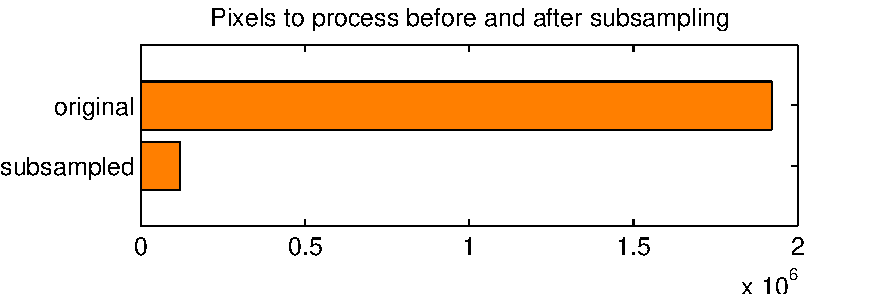
\includegraphics[width=\columnwidth]{pixel_reduced.pdf}
    \caption{Number of pixels in original and subsampled images}
    \label{fig:pixel_reduced}
\end{figure}

We then divide all the training images into a \textbf{training} set and a \textbf{validation} set (shown in Fig.\ref{fig:data_split}, with $80\%$ and $20\%$ in each. That is approximately $40$ images for training and $10$ images for testing, among all $50$. We also notice the fact that there are $10$ distinct distances of the barrel, so we split randomly in each distance category $4$ images to the training set and $1$ image to the validation set. This step is for the purpose of \textbf{model selection} with \textbf{cross validation} in the training phase later.

\begin{figure}[H]
  \centering
  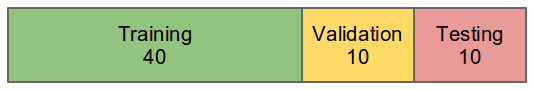
\includegraphics[width=\columnwidth]{data_split.png}
    \caption{Split all images into $80\%$ training and $20\%$ testing}
    \label{fig:data_split}
\end{figure}

As suggested in the project write-up, the default RGB colorspace is not recommended, as it has problems with different lighting condition. We then explore some other colorspace options that are supported in MATLAB. The colorspaces that are being inspected are \textbf{RGB}, \textbf{YCbCr}, \textbf{L*a*b} and \textbf{HSV}. We use $5$ images with distance $1$ to generate the 3D scatter plot in different colorspaces (shown in Fig.\ref{fig:cspace}). \red{Red} dots are pixels from the barrel while dots in other colors are pixels from the rest of the images. As can be seen from the figure, the \textbf{L*a*b} and \textbf{YCbCr} are much better than the rest colorspace in the sense that they have more concentrated clusters.

\begin{figure}[H]
  \centering
  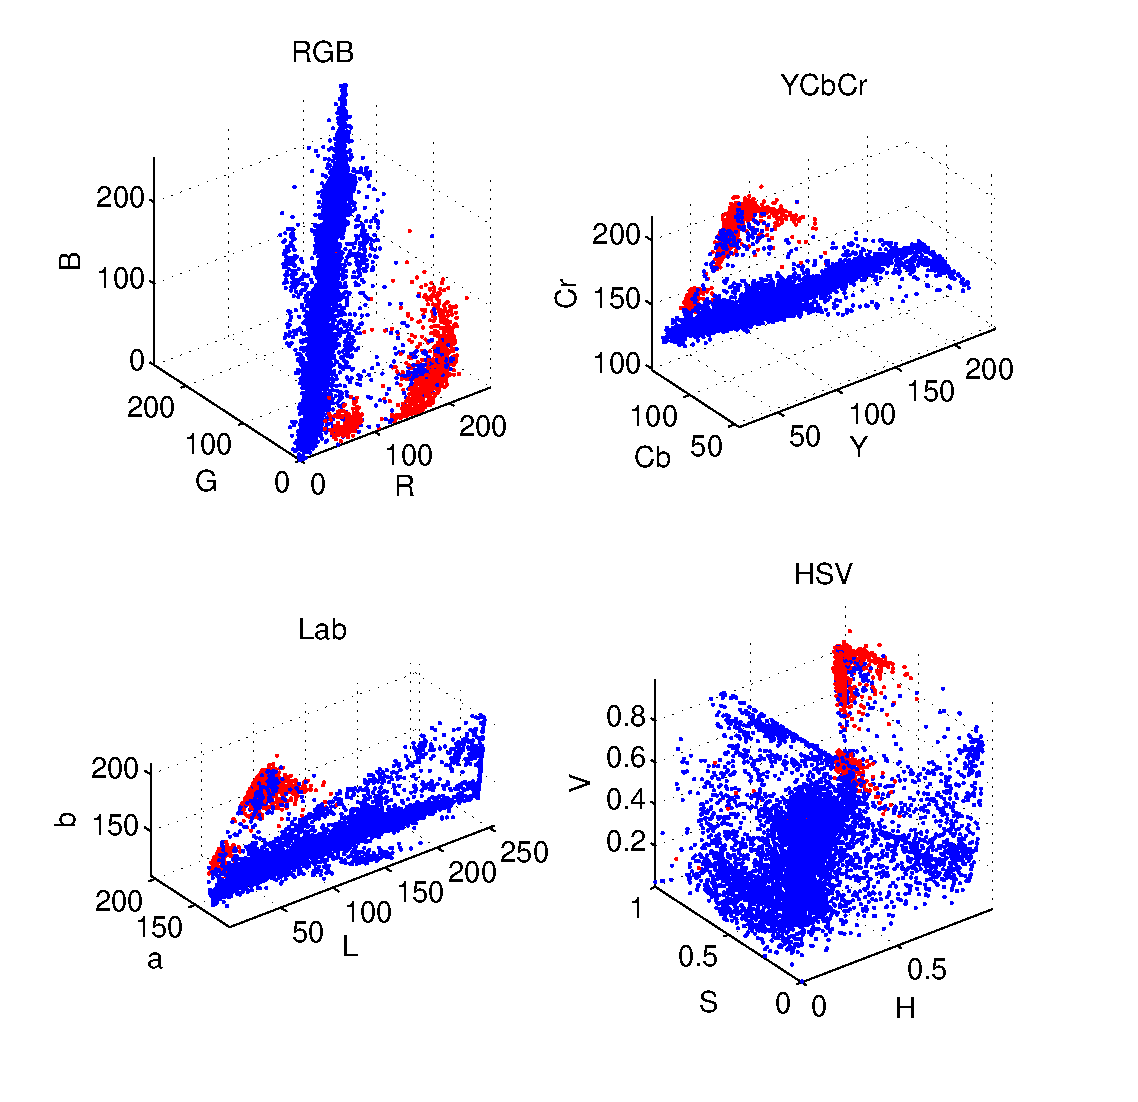
\includegraphics[width=\columnwidth]{cspace.pdf}
    \caption{3D scatter plot for different color spaces}
    \label{fig:cspace}
\end{figure}

A closer look at the two colorspace reveals that pixels in the \textbf{L*a*b} colorspace that represent the red barrel are more concentrated than the rest colospaces (shown in Fig.\ref{fig:cspace_2d}. Thus we pick L*a*b and convert all RGB images to that colorspace. 

\begin{figure}[H]
  \centering
  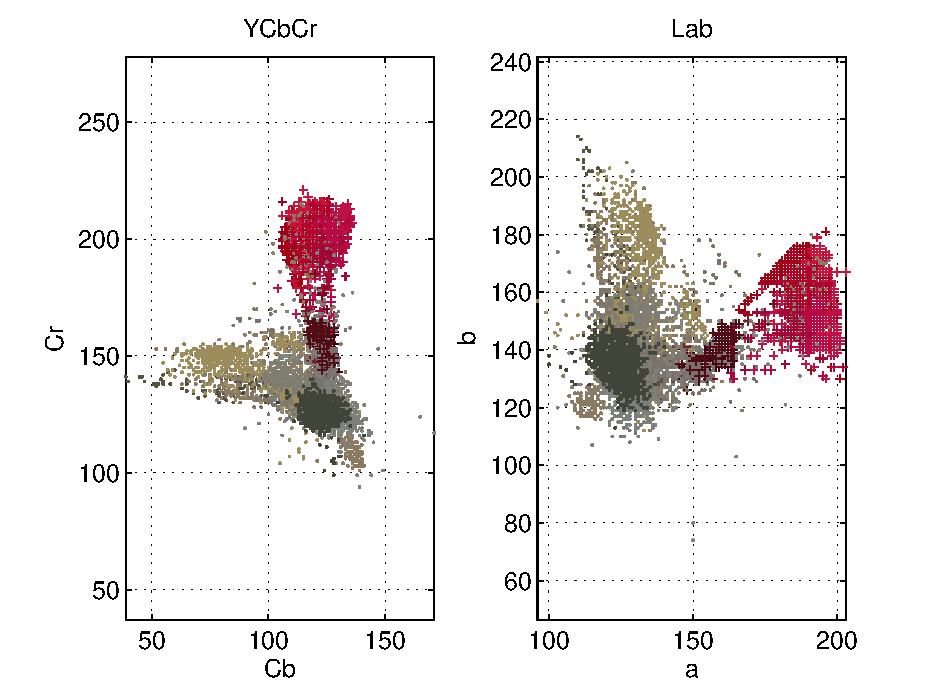
\includegraphics[width=\columnwidth]{cspace_2d.pdf}
    \caption{2D scatter plot on the 2 color channels of L*a*b and YCbCr}
    \label{fig:cspace_2d}
\end{figure}

Also, we notice that in the 2d plot of L*a*b, there are two clusters of red pixels. The darker but smaller cluster is closer to non-barrel pixels while the lighter ones are far away. This is due to the fact that the images are taken under different lighting conditions. This observation encourages us to learn maybe two models for light and dark conditions or maybe to use a \textbf{Gaussian Mixture Model}. An example of confusing images under different lighting conditions are shown in Fig.\ref{fig:confusing}.

\begin{figure}[H]
  \centering
  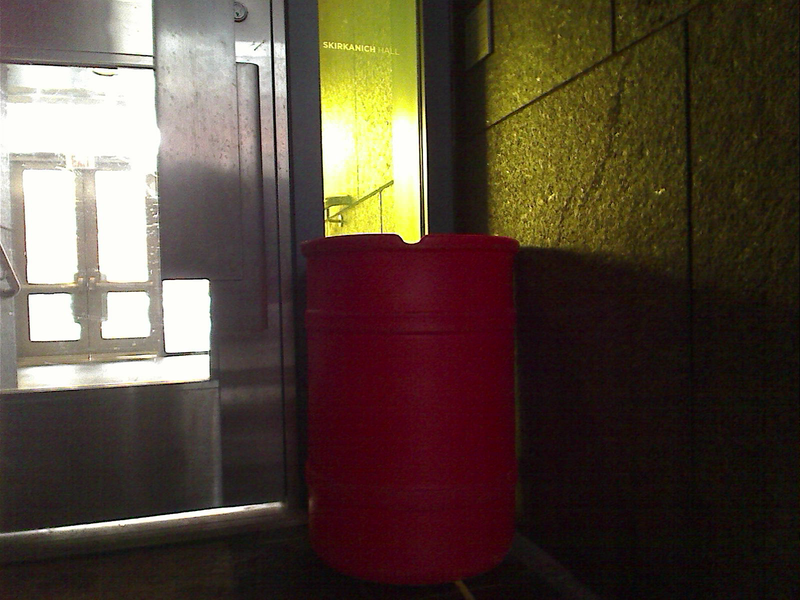
\includegraphics[width=0.4\columnwidth]{barrel_dark.png}
  \;\;\;
  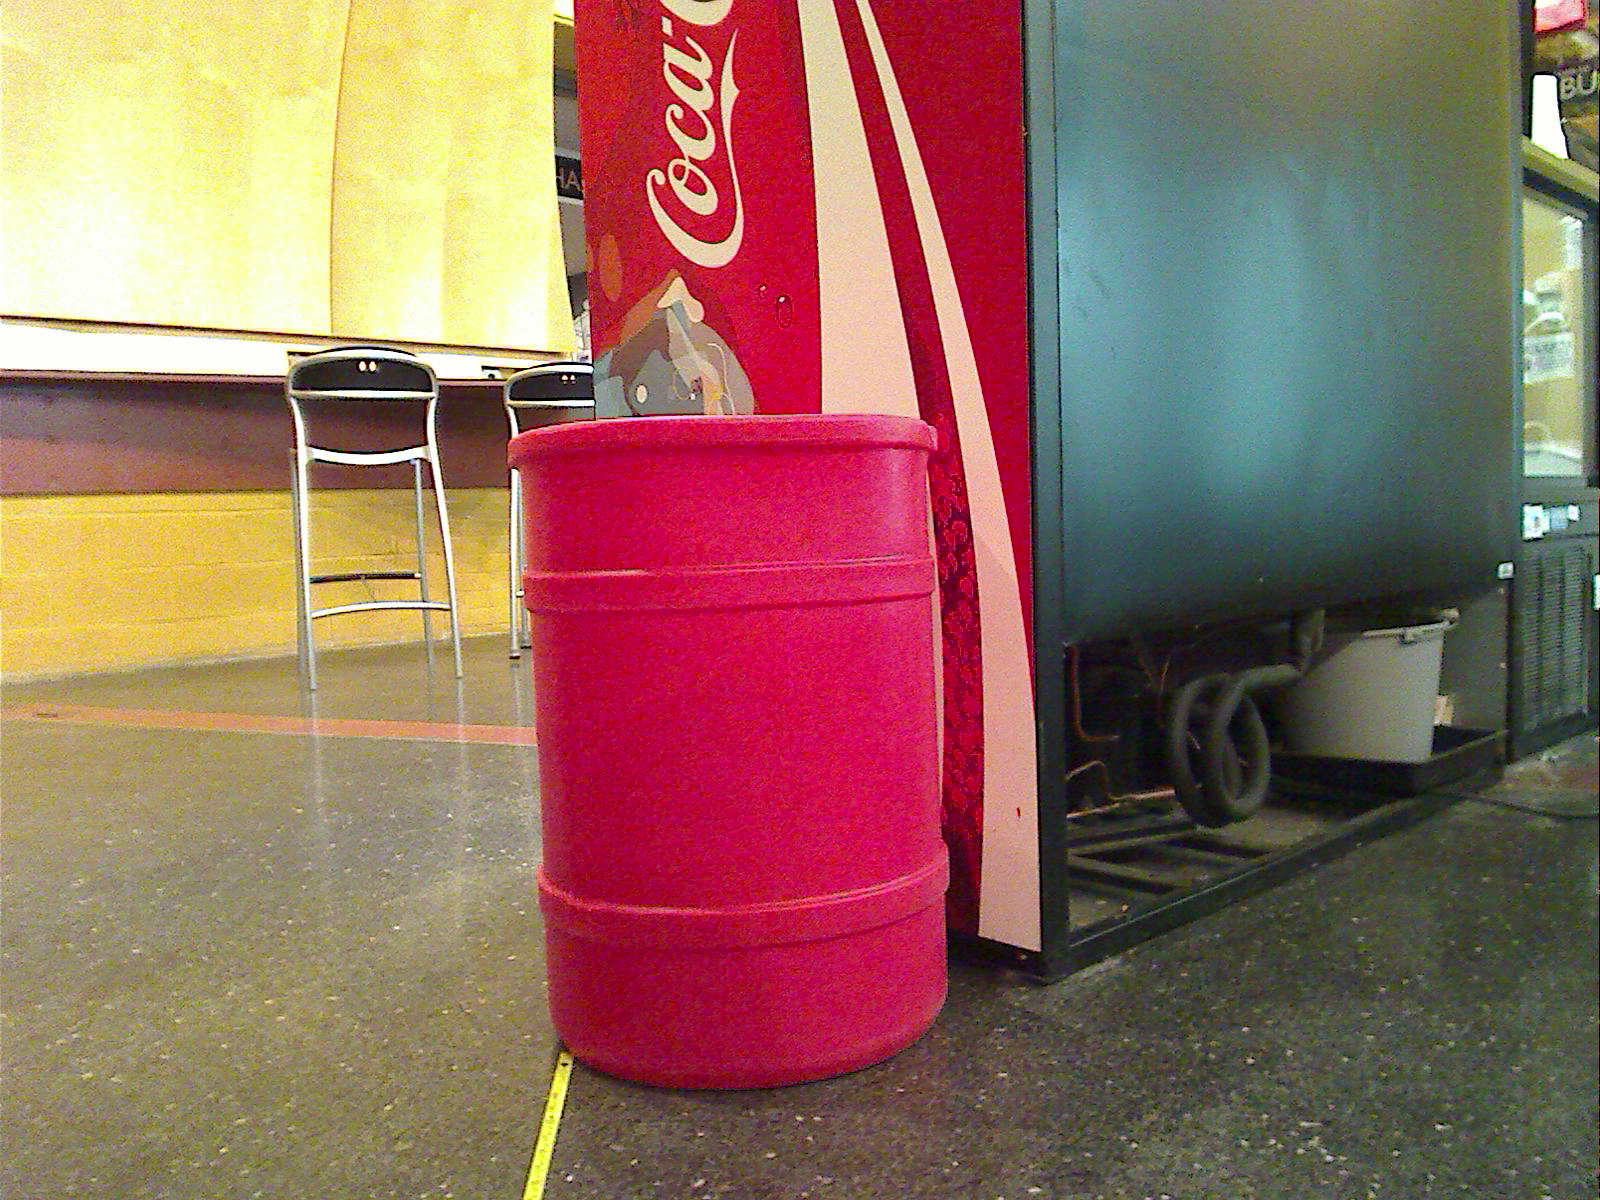
\includegraphics[width=0.4\columnwidth]{barrel_red.png}
  \caption{Images under different lighting conditions. \label{fig:confusing}}
\end{figure}

Finally, in order to tell our algorithm which part of the image contains the barerl, we hand labelled all the barrels in training images and creating a mask for each image (shown in Fig.\ref{fig:barrel_mask}).

\begin{figure}[H]
  \centering
  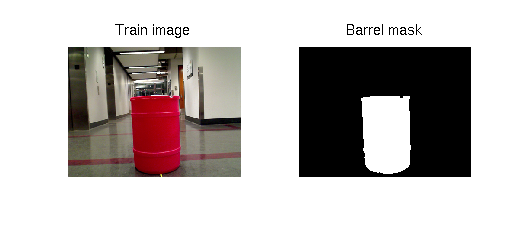
\includegraphics[width=\columnwidth]{barrel_mask.png}
    \caption{Barrel mask for each training image}
    \label{fig:barrel_mask}
\end{figure}

%----------------------------------------------------------------------------------------
%	METHODS
%----------------------------------------------------------------------------------------

\section{METHODS}
After pre-processing the data, I start playing with different methods and models. Here I describe the learning and predicting workflow that I use for color segmentation and barrel detection.

\subsection{Barrel Shape Model}
Since we already have a black-white image to mask the barrel, we could learn some useful information from that. We looked at various properties of the part of mask being labelled and decided to use the aspect ratio and percentage of filled pixels to model the barrel. From the training image, we extract all those information and build a 2D Gaussian distribution. And for any new mask coming in, we will be able to tell the probability of it being a barrel or not. The equations used for estimating such a multivariate gaussian is shown in (Eq.\ref{eq:mle1} and \ref{eq:mle2}) and the result are shown in Fig.\ref{fig:barrel_model}.

\begin{equation}
\mu_{MLE} = \frac{1}{N}\sum_{i=1}^N\mathbf{x}^i
\label{eq:mle1}
\end{equation}
\begin{equation}
\Sigma_{MLE} = \frac{1}{N}\sum_{i=1}^N(\mathbf{x}-\mu)(\mathbf{x}-\mu)^{\top}
\label{eq:mle2}
\end{equation}

\begin{figure}[H]
  \centering
  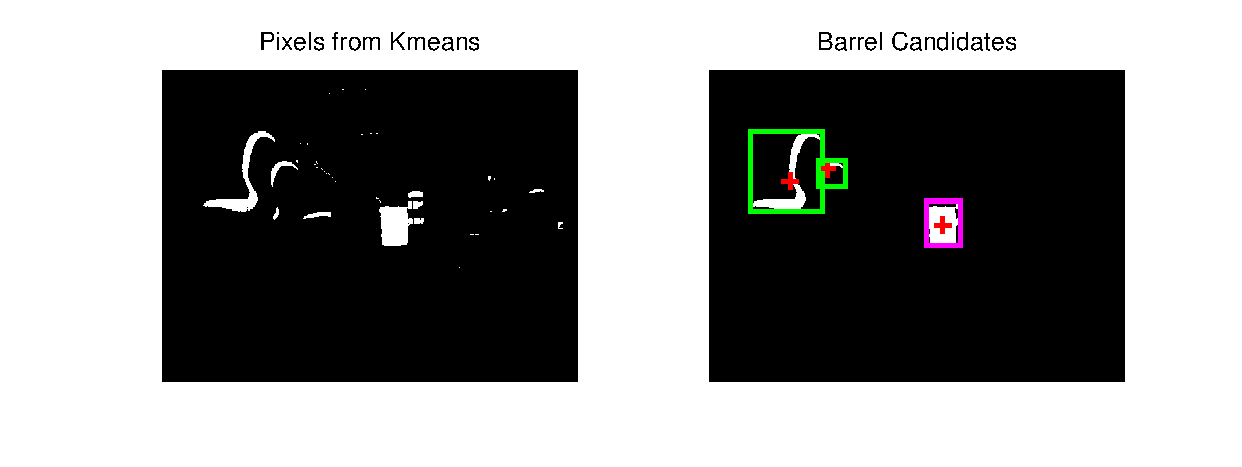
\includegraphics[width=\columnwidth]{barrel_model.pdf}
    \caption{Using barrel model to select the most possible shape}
    \label{fig:barrel_model}
\end{figure}


\subsection{Distance Model}
For distance estimation, we adopt the simple approach of ridge regression with 3 features: height and width of the bounding box and square root of the area of the mask. The equations used for estimating such a ridge regression is shown in (Eq.\ref{eq:ridge}).

\begin{equation}
\mathbf{w}_{MLE} = (\mathbf{X}\mathbf{X}^\top + \lambda \mathbf{I})^{-1}\mathbf{X}^\top \mathbf{y}
\label{eq:ridge}
\end{equation}

\subsection{K-means Clustering}
For color segmentation, we first use the K-means algorithm on channel a and b of the lab colorspace image. We start with an initial clusters of 4 and keep increasing until we get a shape that has a high probability of being a barrel. For most of the image, the barrel can be segmented with in 1 or 2 iterations or K-means. For those harder cases, it can also be found at higher cluster number. Since there are two different lighting conditions, we compare the L channel of each image to a lightness threshold and based on that we select which cluster to be the barrel or red (shown in Fig.\ref{fig:kmeans.png}).

\begin{figure}[H]
  \centering
  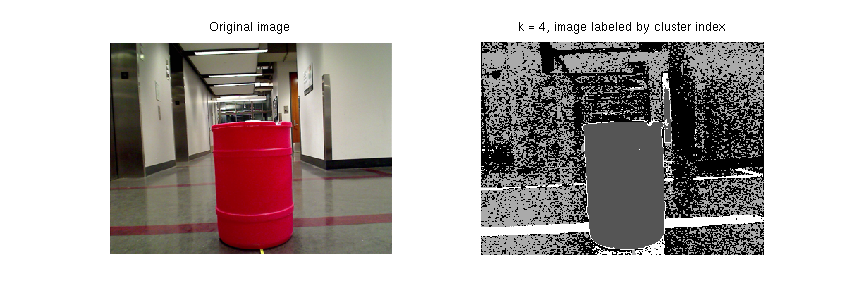
\includegraphics[width=\columnwidth]{kmeans.png}
    \caption{Sample results of K-means}
    \label{fig:kmeans}
\end{figure}

\subsection{Gaussian Mixture Model}
When K-means fails, GMM comes in. Since K-means can do good enough on most of the images, we use GMM only for those cases where K-means cannot detect a good shape of barrel. We use all the pixels in the aforementioned masks to train a GMM model for red with 2 mixtures. Then for each given image, we calculate the probability of them being red. We then threshold and normalize them to create a black white image that is similar to what we get from K-means. Then we apply the same process to the black white image and get the most possible shape to be a barrel (shown in Fig.\ref{fig:gmm}).

\begin{figure}[H]
  \centering
  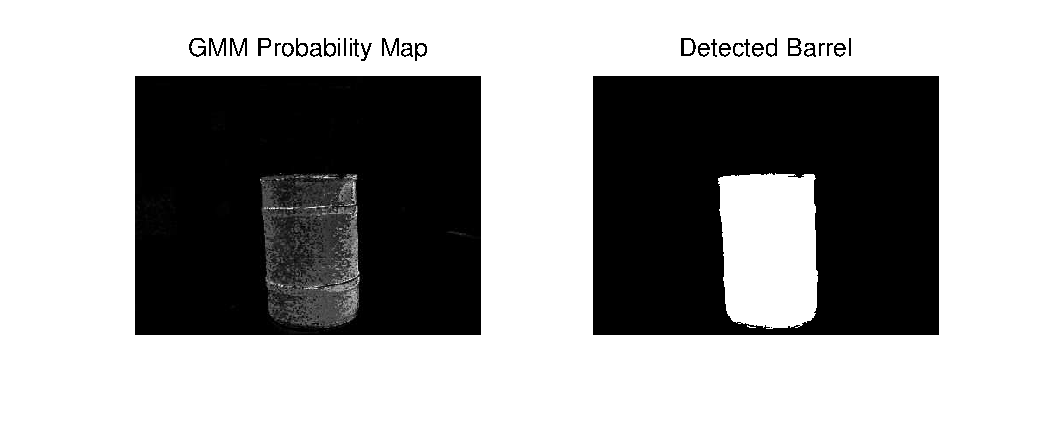
\includegraphics[width=\columnwidth]{gmm.pdf}
    \caption{Sample results of GMM}
    \label{fig:gmm}
\end{figure}

%----------------------------------------------------------------------------------------
%	RESULTS
%----------------------------------------------------------------------------------------

\section{DISCUSSION}

\subsection{RESULTS}
In this section we show some of results detected by our model. We first look at all the estimated depth result (shown in \ref{fig:depth}).

\begin{figure}[H]
  \centering
  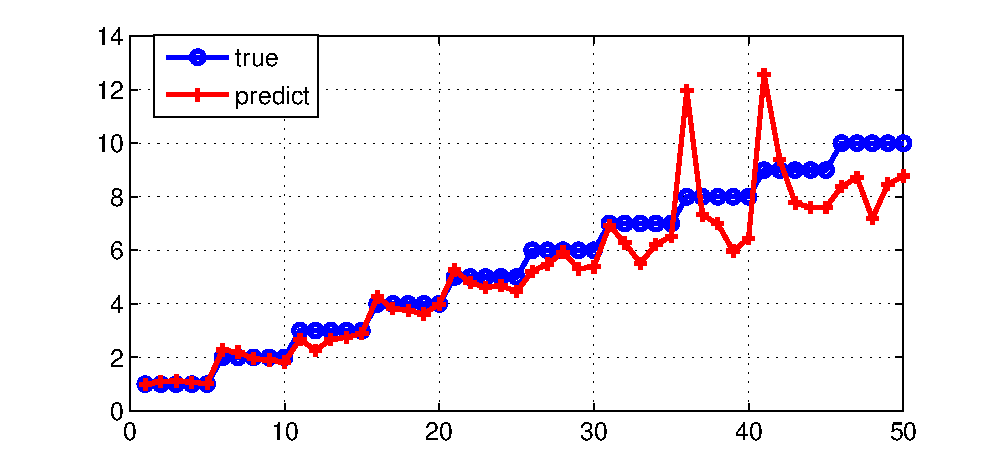
\includegraphics[width=\columnwidth]{result.pdf}
    \caption{Estimate depth vs. true depth}
    \label{fig:depth}
\end{figure}

We then look at some of the detected barrels.

\begin{figure}[H]
  \centering
  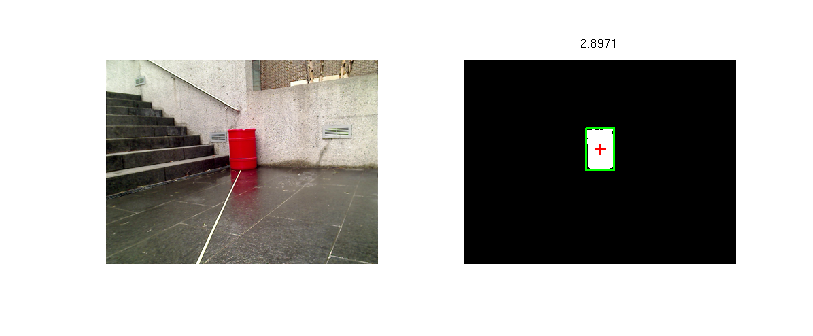
\includegraphics[width=\columnwidth]{t20.png}
    \caption{Sample detected barrel}
    \label{fig:t20}
\end{figure}

\begin{figure}[H]
  \centering
  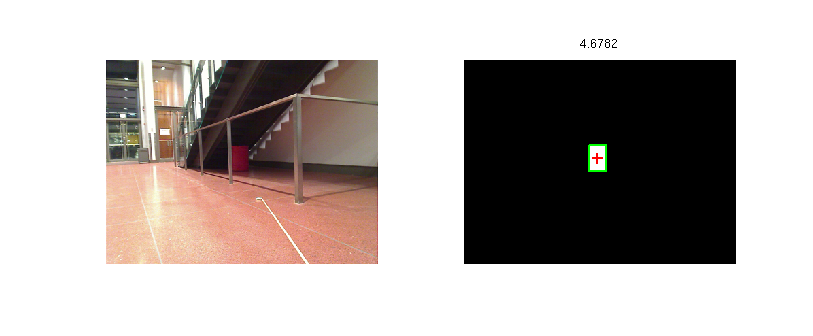
\includegraphics[width=\columnwidth]{t30.png}
    \caption{Sample detected barrel}
    \label{fig:t30}
\end{figure}

\begin{figure}[H]
  \centering
  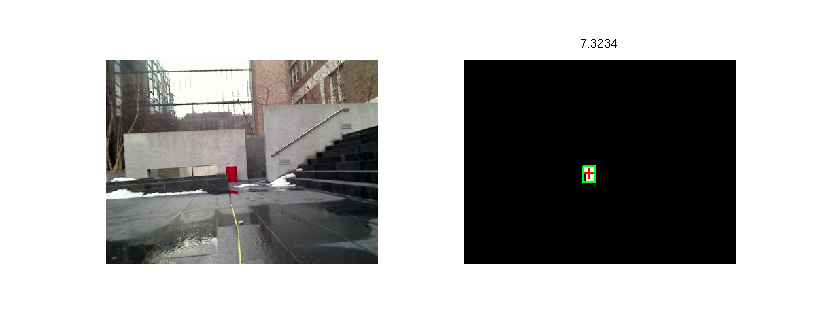
\includegraphics[width=\columnwidth]{t40.png}
    \caption{Sample detected barrel}
    \label{fig:t40}
\end{figure}

\subsection{IMPROVEMENT}
There are several improvements that can be made to this project.
\begin{enumerate}
\item Increase the speed of GMM.
\item Train a better model on the barrel.
\item Train a better mode for distance estimation.
\end{enumerate}

%----------------------------------------------------------------------------------------
%	REFERENCE LIST
%----------------------------------------------------------------------------------------

%\begin{thebibliography}{99} % Bibliography - this is intentionally simple in this template
%
%\bibitem[Figueredo and Wolf, 2009]{Figueredo:2009dg}
%Figueredo, A.~J. and Wolf, P. S.~A. (2009).
%\newblock Assortative pairing and life history strategy - a cross-cultural
%  study.
%\newblock {\em Human Nature}, 20:317--330.
% 
%\end{thebibliography}

%----------------------------------------------------------------------------------------

\end{multicols}

\end{document}